\section{High Threshold Cerenkov Counter (HTCC)}

\subsection{Geometry}

The HTCC geometry is implemented through the native gemc geometry API. The elliptical mirrors are made through a subtraction of
two G4Ellipsoid. They are contained inside an HTCC mother volume made with a G4Polycone, see \F{htccGeometry}.
The faces of the PMT are the sensitive volumes, associated with the quartz-glass material and associated with the htcc digitization routine.

The refractive index of the $CO_2$ and its transparency is included in the material optical properties and taken
into account during the geant4 transportation of the phtotons.

The mirror and winston cones reflectivities are associated with the mirror optical properties and are taken into
account and taken into account during the geant4 transportation of the phtotons.

The quartz window PMT quantum efficiency are associated with the PMT face optical properties and are taken into account in
the digitization routine.


\begin{figure}
	\centering
	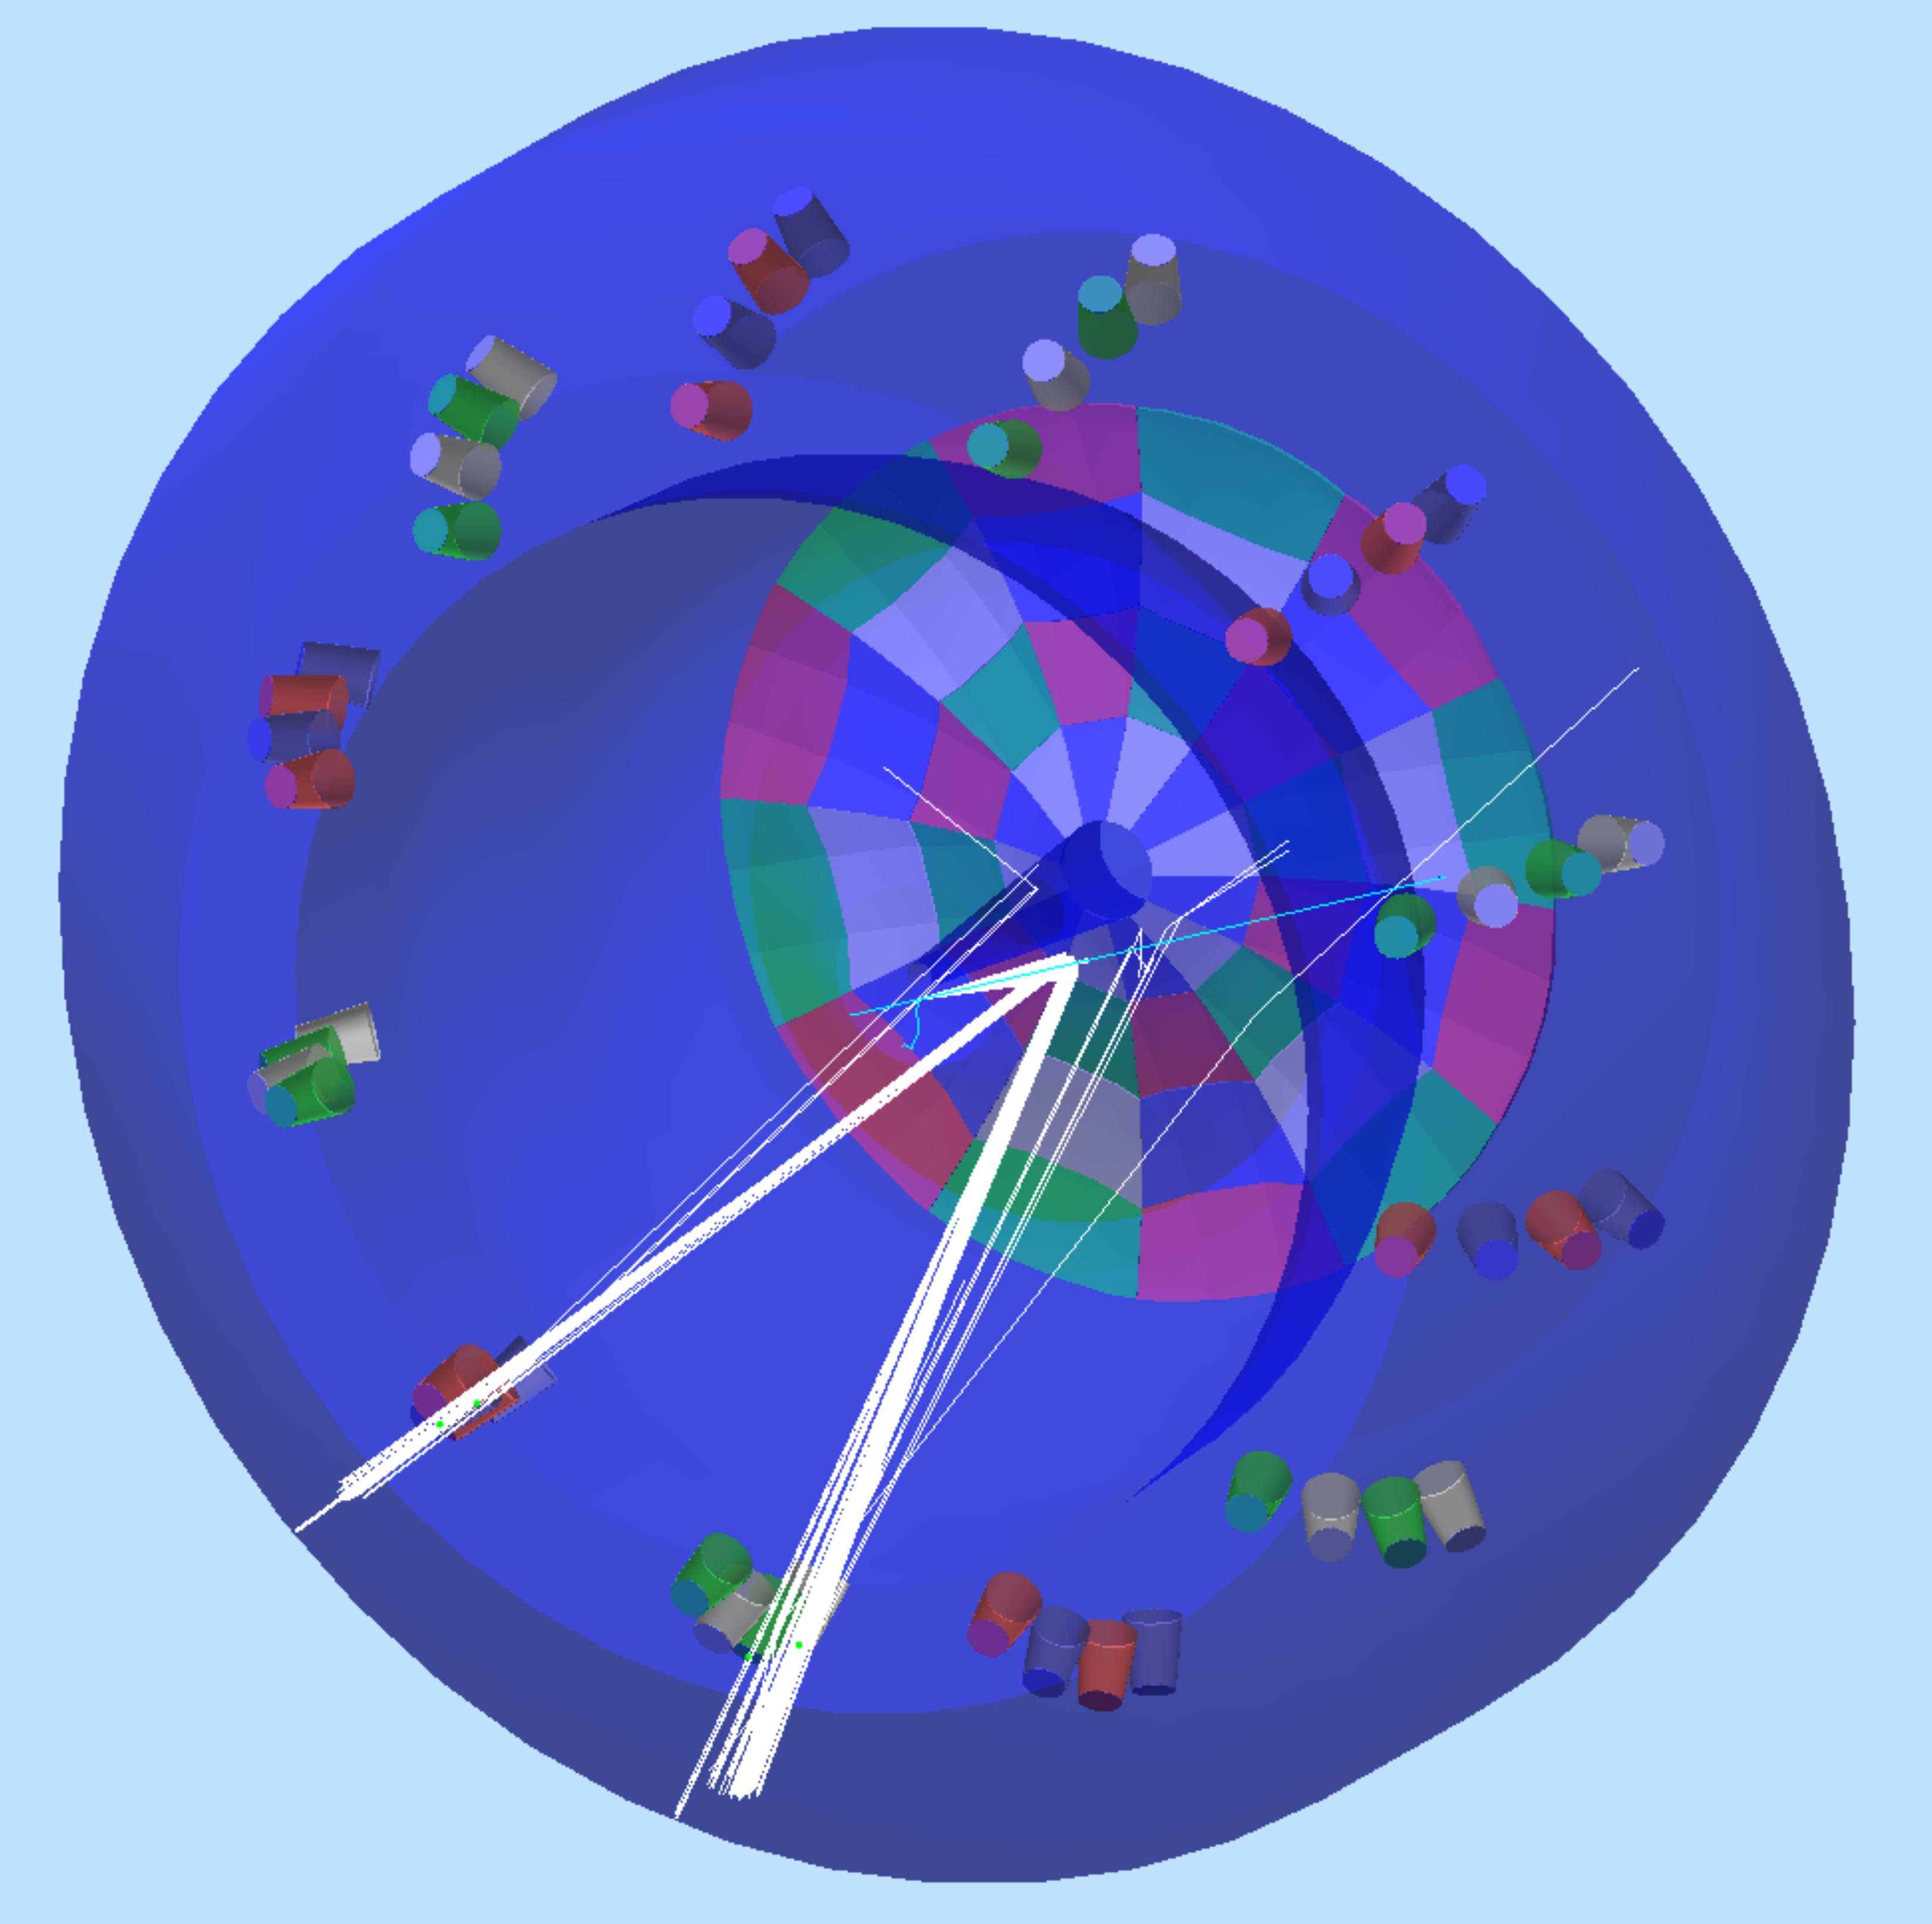
\includegraphics[width=0.95\columnwidth,keepaspectratio]{img/htccGeometry.png}
	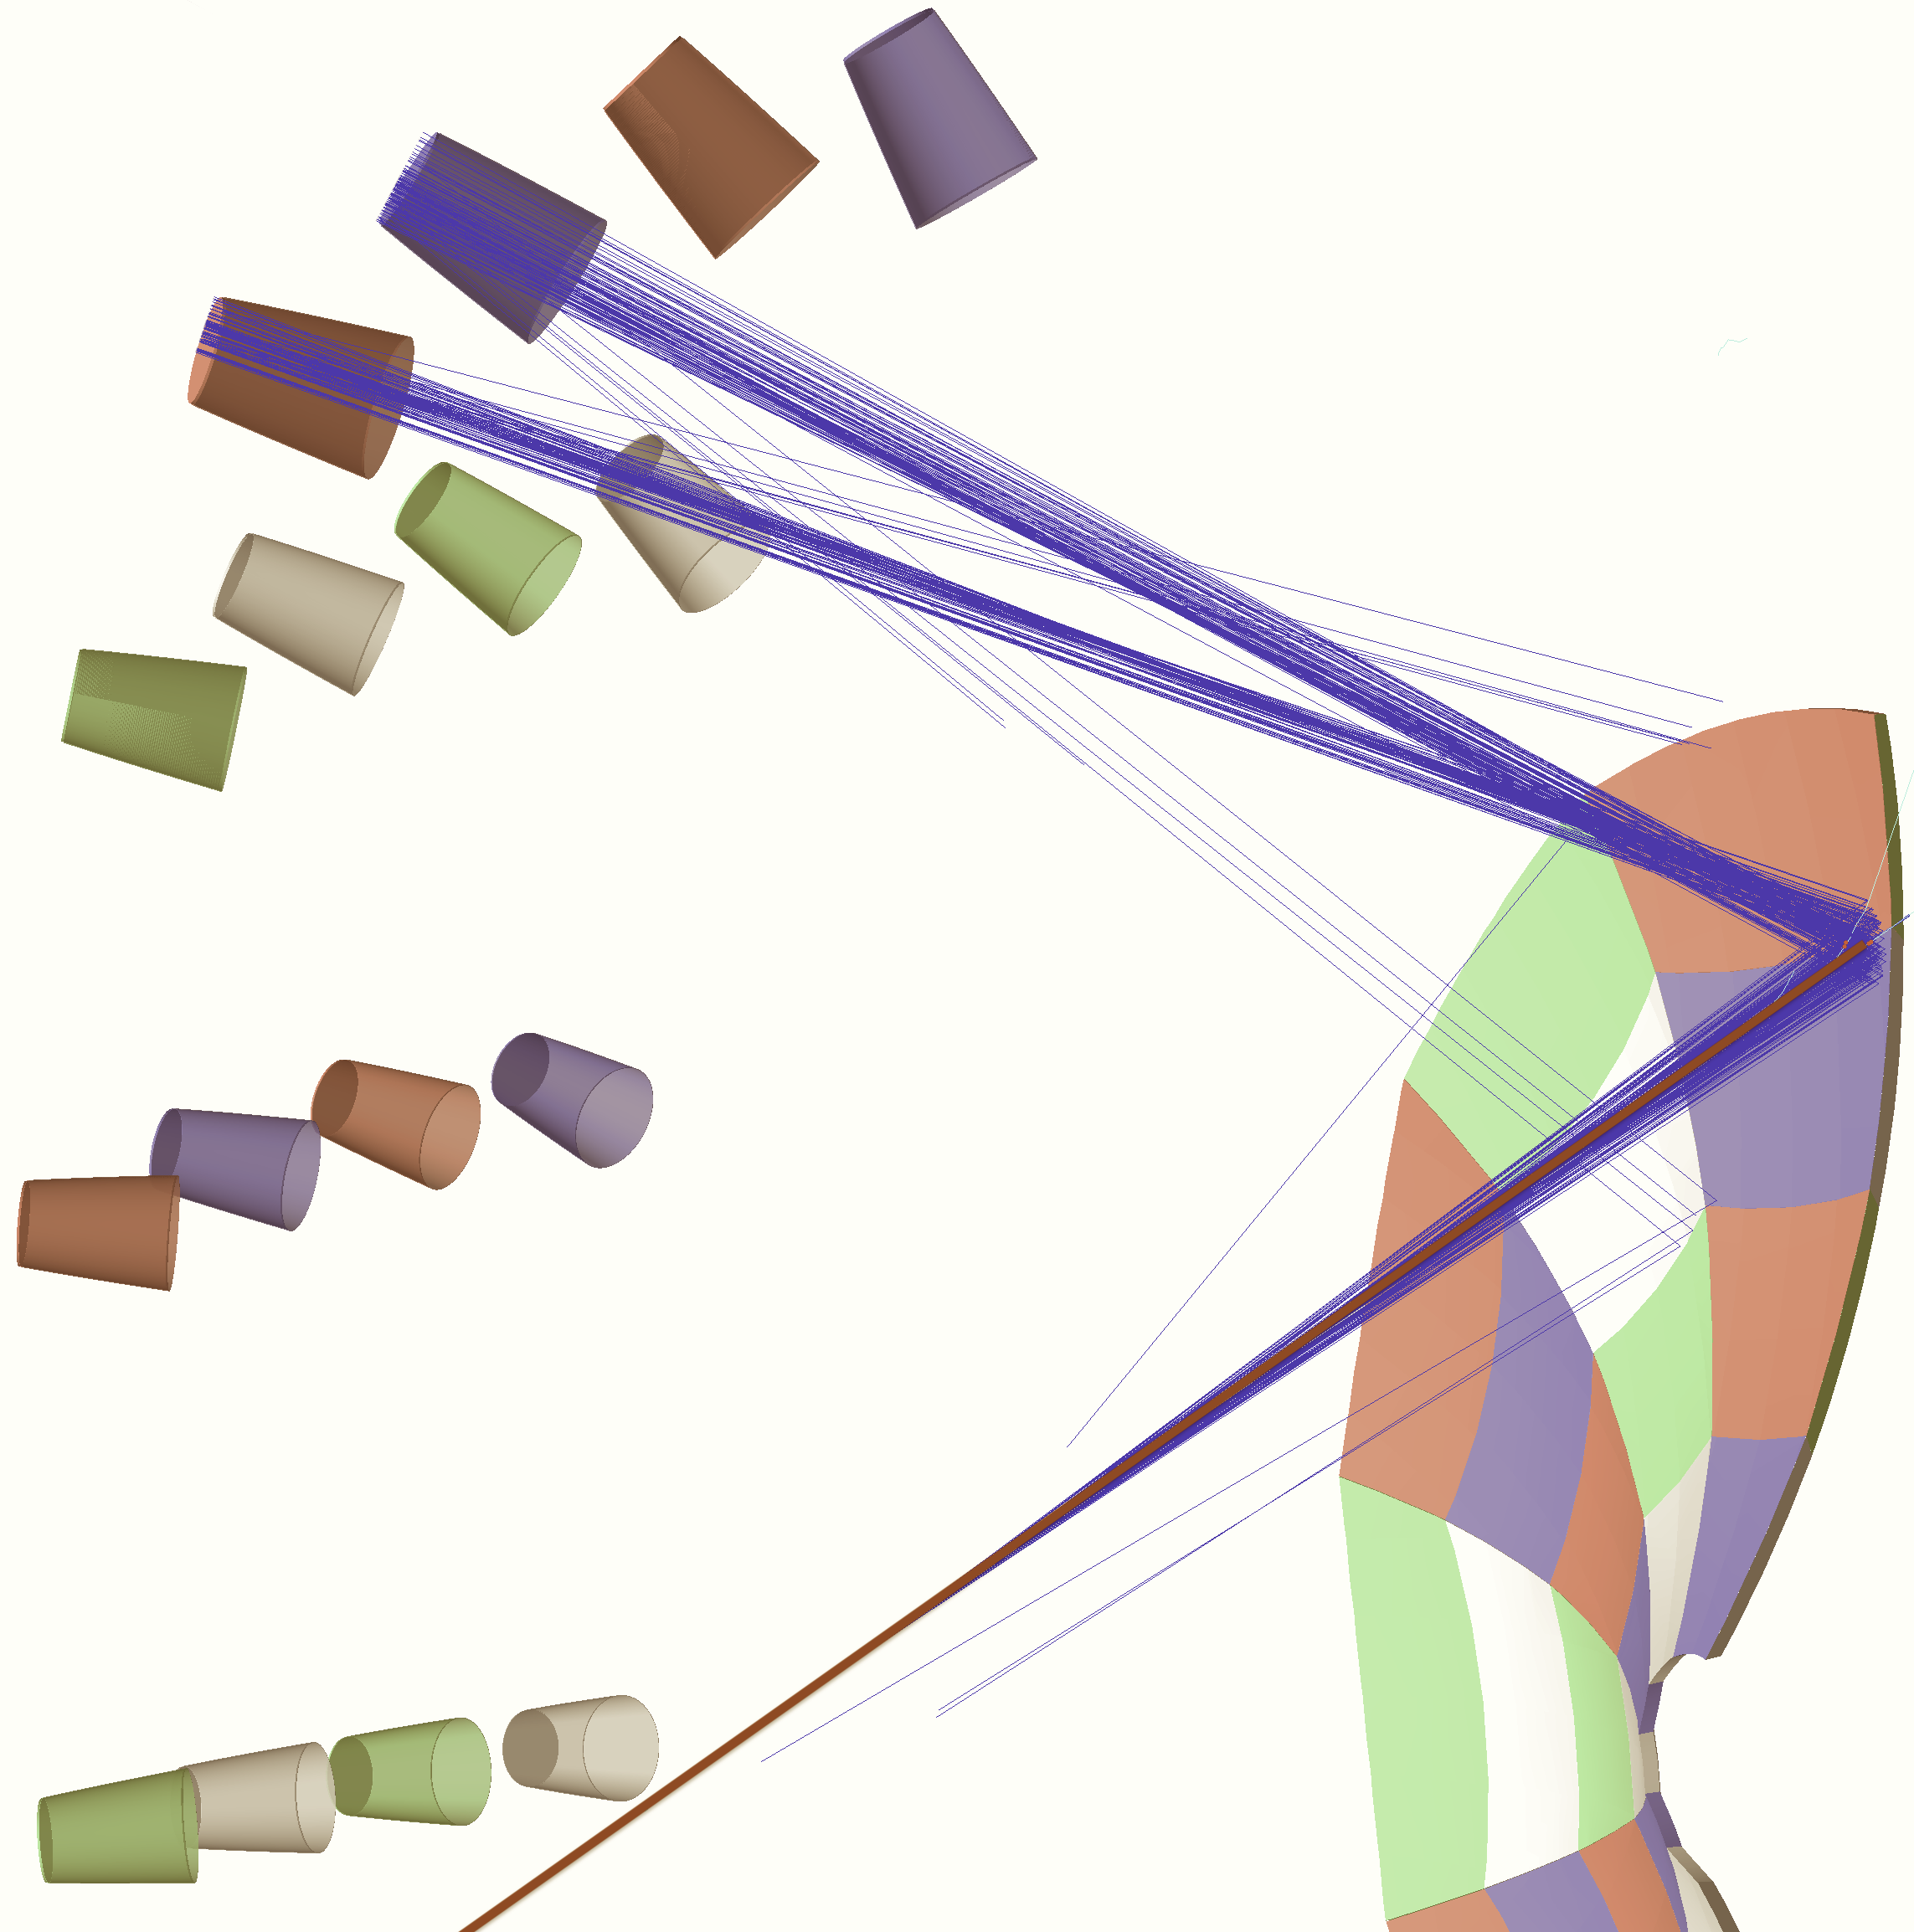
\includegraphics[width=0.95\columnwidth,keepaspectratio]{img/htccDetail.png}
	\caption{Top: overall view of the CND detector. Three layers of scintillators are placed at increasing z. Pairs of scintillators
            are connected through a scintillator u-shaped junction. Bottom: enlarged view of the junctions. }
	\label{fig:htccGeometry}
\end{figure}


\subsubsection{Geometry Git Location}
The github location of the gemc perl api script is \url{https://github.com/gemc/detectors/tree/master/clas12/htcc}.



\subsection{Digitization}
Photons that impinged on the PMT faces are processed. For each photon collected undergoes the quantum efficiency algorithm at its
wavelength to decided if it's finally detected.

\subsubsection{Timing}

The time average of all the photons is saved in the output after a time shift coming from the calibration database.


\subsubsection{Summary of CCDB Table used}
\begin{itemize}
	\item /calibration/htcc/status
	\item /calibration/htcc/time
	\item /daq/tt/htcc:
\end{itemize}

\subsection{Digitized Bank}
The digitized output bank has $ID=600$, and the variables are summarized in Table \ref{tab:htccBank}

\begin{table}[h]
	\begin{center}
		\begin{tabular}{| c | c | c |}
			\hline \hline
			Variable         & Description  & Tag  \\
			\hline
           sector  &                                     clas12 sector  &    1   \\
             ring  &                                       theta index  &    2   \\
             half  &                                       half-sector  &    3   \\
             nphe  &                          number of photoelectrons  &    4   \\
             time  &                           average time of the hit  &    5   \\
             hitn  &                                        hit number  &   99   \\
			\hline \hline
		\end{tabular}
	\end{center}
	\caption{The digitized HTCC bank}\label{tab:htccBank}
\end{table}

\subsubsection{Time Window}
The timewindow of the HTCC is set to 5 ns.

\subsubsection{Background merging algorithm}

\subsubsection{Process Routine Git Repository Location}
The HTCC hit process routine location in git is \url{https://github.com/gemc/source/blob/master/hitprocess/clas12/htcc_hitprocess.cc}
